% !TeX spellcheck = en_AM
\section{Implicit Surfaces}

In one spatial dimension a line can be enclosed by two points to form a sub-domain. For example the two points $x = -1$ and $x = +1$ would split the dimension into three different segments. The segment $(-1, +1)$ represents the inside portion of the domain $\Omega^-$, while the union of other two segments  $(-\infty,-1) \cup (+1,+\infty) $ represents the outside portion $\Omega^+$. The border of the two portions is called interface  $\partial\Omega$. In this example the interface would be represented by the two points $x = -1$ and $x = +1$ \cite{osher:2006:level}.

A similar concept can be applied in two dimensions, defining a surface by using lines as interface, as well as in three dimension, defining a volume and using surfaces as interface. Note that the interface is always one less dimension than the sub-domain it encloses \cite{osher:2006:level}.

\subsection{Implicit functions}

While interfaces can be explicitly defined, it is also possible to define them using implicit functions. An implicit function $\Phi(\vec{x})$ is defined on all points $\vec{x} \in \Re^n$. If $\vec{x}$ lies on the interface the \gls{sdf} returns 0. For points in $\Omega^-$ the result is a negative value, while for $\Omega^+$ it is positive value \cite{osher:2006:level}. Formally:
\begin{itemize}
	\item $\forall \vec{x} \in \partial\Omega,  \Phi(\vec{x}) = 0$ 
	\item $\forall \vec{x} \in \Omega^-,  \Phi(\vec{x}) < 0$
	\item $\forall \vec{x} \in \Omega^+,  \Phi(\vec{x}) > 0$
\end{itemize}

The implicit function version of the previous example would be $\Phi(x) = x^2 - 1$, which gives 0 for the case $x = -1$ and $x = +1$.
In two dimensions the implicit function $\Phi(\vec{x}) = x^2 + y^2 - 1$ defines a circle, while in three dimensions  $\Phi(\vec{x}) = x^2 + y^2 + z^2 - 1$ defines a sphere. $x$, $y$ and $z$ are the respective components of $\vec{x}$ \cite{osher:2006:level}.

\subsection{Normal and gradient}

A useful property of an implicit function is its gradient. The gradient will always point in the direction where the value of $\Phi$ increases. For a point on the interface this is also the direction of its normal. The gradient $\vec{\nabla}\phi$ is defined as a vector, the components of which are the resulting value of the partial differential of $\phi$, differentiated in its corresponding dimension\cite{osher:2006:level}. Formally: $\vec{\nabla}\phi = (\frac{\partial\phi}{\partial x},\frac{\partial\phi}{\partial y},\frac{\partial\phi}{\partial z})$ 

To create the unit normal of a point on the interface we need to normalize the gradient, resulting in the following function: $\vec{N}(\vec{x}) = \frac{\vec{\nabla}\phi(\vec{x})}{|\vec{\nabla}\phi(\vec{x})|}$. In addition this does not only work for points on the interface, but for any point, with a few exceptions where the denominator becomes zero. For $\Phi(x) = x^2 - 1$ and its derivative $\Phi(x)' = 2x$, the normal of $x = 0$ would not be defined \cite{osher:2006:level}.

In cases where the exact derivative cannot be used, it can be approximated. Some examples for approximations are:
\begin{itemize}
	\item forward difference:  $\frac{\partial\phi(\vec{x})}{\partial x} \approx \frac{\phi(x+\Delta, y, z) - \phi(\vec{x})}{\Delta}$
	\item backward difference: $\frac{\partial\phi(\vec{x})}{\partial x} \approx \frac{\phi(\vec{x}) - \phi(x-\Delta, y, z)}{\Delta}$
	\item central difference: $\frac{\partial\phi(\vec{x})}{\partial x} \approx \frac{\phi(x+\Delta, y, z) - \phi(x-\Delta, y, z)}{2*\Delta}$
\end{itemize}

The versions for the partial derivatives for y, z are analogous to the above examples \cite{osher:2006:level}.


\subsection{Boolean Operations}
\label{section:boolean}
Another useful property of implicit functions is that they can be easily composed with other implicit functions and Boolean operations. For example the union of the interior regions from two implicit functions $\phi_1(\vec{x})$ and $\phi_2(\vec{x})$ can be described as another implicit function $\phi(\vec{x})$ such as: $\phi(\vec{x}) = min(\phi_1(\vec{x}), \phi_2(\vec{x}))$. Other Boolean operations of the implicit functions' interior regions are:
 
\begin{itemize}
	\item Intersection:  $\phi(\vec{x}) = max(\phi_1(\vec{x}), \phi_2(\vec{x}))$
	\item Complement or Negation: $\phi(\vec{x}) = -\phi_1(\vec{x})$ 
	\item Subtracting $\phi_2(\vec{x})$ from $\phi_1(\vec{x})$ :  $\phi(\vec{x}) = max(\phi_1(\vec{x}), -\phi_2(\vec{x}))$
\end{itemize}

\subsection{Signed Distance Functions}
\Glspl{sdf} are implicit functions, the absolute value of which is equal to the distance between $\vec{x}$ and its nearest point on the interface. Formally:  $|\Phi(\vec{x})| = min(|\vec{x} - \vec{y}|) \, \forall \, \vec{y} \in \partial\Omega$. They possess the property that the length of their gradient is almost always 1, or formally  $|\nabla\phi| = |(\frac{\partial\phi}{\partial x},\frac{\partial\phi}{\partial y},\frac{\partial\phi}{\partial z})| = 1$. However, this is only true for the general case, but not for points which are equidistant to two or more points on the interface \cite{osher:2006:level}.

If the general case is assumed, for a given point $\vec{x}$ the nearest point on the interface $\vec{y}$ can be calculated using the following formula: $\vec{y} = \vec{x} - \phi(\vec{x}) * \vec{N}(\vec{x}) $

This can be simplified as  $\vec{N}(\vec{x}) = \frac{\nabla\phi(\vec{x})}{|\nabla\phi(\vec{x})|}$ and $|\nabla\phi| = 1$, resulting in 
$\vec{y} = \vec{x} - \phi(\vec{x}) * \nabla\phi(\vec{x}) $ \cite{osher:2006:level}

\section{Ray tracing Implicit Surfaces}
Ray tracing is a rendering technique, which creates an image by casting rays into the scene. For each pixel a ray is cast and checked for intersections with objects in the scene. The pixel's color is the color of that intersected object at the corresponding intersection point. Actual ray tracing may involve more than just casting one ray per pixel, but this will be left out for simplicity. The main problem that needs to be solved for ray casting, is to be able to intersect the ray with the objects contained in a scene \cite{bungartz:2013:einfuhrung}.

\subsection{Mathematical Root Finding}
One method for finding the intersection is by directly calculating it. Let $r(t) = r_0 + t* \vec{r_d}$ be the ray's equation, where $r_0$ is the ray's origin and $\vec{r_d}$ the normalized direction of the ray. Then by plugging the ray equation $r : \mathds{R} \rightarrow \mathds{R}^{3} $ into the implicit function $\phi : \mathds{R}^{3} \rightarrow \mathds{R} $, the composite function $F : \mathds{R} \rightarrow \mathds{R}$ is created. The least positive $t$ where $F(t) = 0$ (root of $F$) can then be inserted into the ray's equation to calculate the intersection point\cite{hart:1996:sphere}.

However, for more complicated functions it may not be possible to calculate the root. One solution is to use Newton’s method to find the roots. However, this only works if the functions is derivable \cite{hart:1996:sphere}. There also exist other methods to find the roots such as interval analysis \cite{mitchell:1990:robust}.

\subsection{Ray Marching}
Ray marching is an iterative algorithm to find the first intersection of a ray which is cast into a scene. The algorithm consists of $\vec{x_i}$ and $\vec{ \Delta x}$, which are the current location and the increment respectively. The initial value for $\vec{x_0}$ is the ray's origin. $\vec{ \Delta x}$ is a fixed vector of a chosen length, which points into ray's direction. With each step the algorithm checks whether $\vec{x}$ is currently inside an object. For instance this could be done with a lookup in a density map or the evaluation of a function. If $x$ is not inside an object increment $\vec{\vec{x}}$ by $\vec{ \Delta x}$. Repeat this step until $\vec{x}$ is inside an object. The intersection lies between the current position  $\vec{x_i}$ and its previous position  $\vec{x_{i-1}}$. This process is aborted if a certain amount of iterations is exceeded or $\vec{x}$ has reached the end of the scene. In this case no intersection was found \cite{tuy:1984:direct, perlin:1989:hypertexture}.

\subsection{Lipschitz continuity, Lipschitz constant and Lipschitz bound}
The Lipschitz continuity, Lipschitz constant and Lipschitz bound are useful properties which are used in the following section. A function fulfils the Lipschitz continuity if and only if the functions is continuous and the magnitude of its derivative is bounded by a constant value. The smallest possible value for this bound Lipschitz constant for that function. For functions, which contain components with known Lipschitz constants, the Lipschitz constant can be overestimated by the Lipschitz bound. A functions Lipschitz bound is greater or equal than its Lipschitz constant. Lipschitz bound of the sum of two functions is equal or less than the sum of Lipschitz bounds of those functions 
\cite{hart:1996:sphere, Heuser:2003}.

\subsection{Sphere tracing}

Sphere tracing can be used to raytrace implicit surfaces, the function of which are Lipschitz continuous. However, the function's derivative does not have to be continuous. It may not even be defined. Sphere tracing finds the first intersection with the implicit surface \cite{hart:1996:sphere}.

Sphere tracing works similar to ray marching. However, instead of a fixed increment it dynamically calculates it using an unbounding sphere. While a bounding sphere would contain an object, an unbounding sphere does not contain any object. The increment is then always set so that its length equals the radius of the unbounding sphere \cite{hart:1996:sphere}. 
Figure \ref{fig:sphere-trace} shows two different sphere traces, the unbounding spheres and how the increment changes each step.

\begin{figure}[!h]
	\begin{center}
	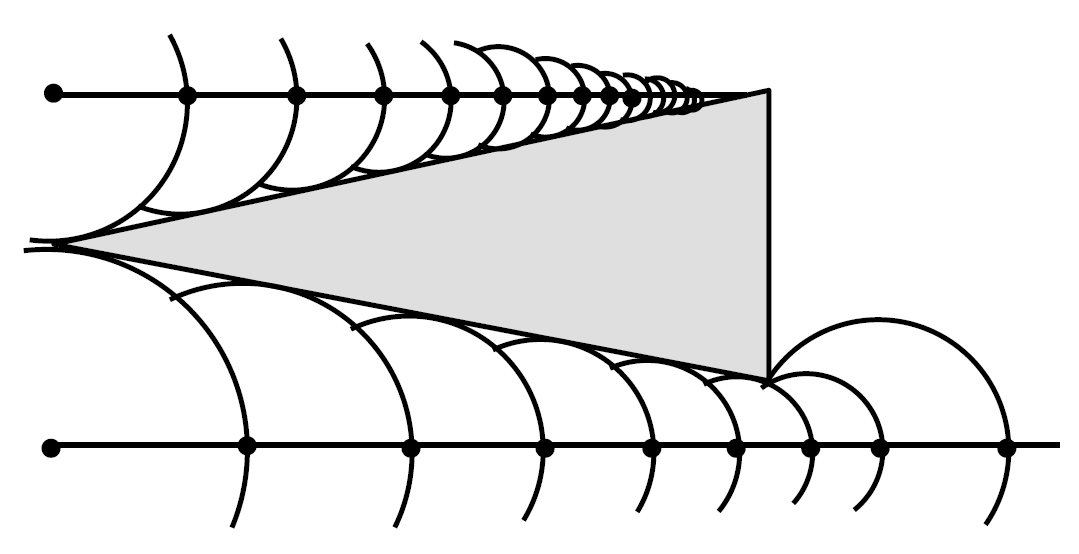
\includegraphics[height=2.5cm]{sphere-trace-hit-and-miss.png}
	\caption{Sphere trace hit and miss \cite{hart:1996:sphere}}
	\label{fig:sphere-trace}
	\end{center}
\end{figure}

The calculation of the unbounding sphere makes use of the Lipschitz continuity. If the implicit surface's function is evaluated at a point and then the point is moved by one unit and evaluated again, the two results cannot differ by more than the function's Lipschitz bound. Thus, if we evaluate the implict surface's function at a given point and divide the result by the Lipschitz bound, we get the radius of the unbounding sphere. The implicit function's surface function will never evaluate to zero, unless the evaluation point is moved at least by the unbounding sphere's radius. \Glspl{sdf} have a Lipschitz Bound of 1. When a Surface is described by  \glspl{sdf}, the the unbounding sphere's radius is equal to the function's evaluation result \cite{hart:1996:sphere}.

\section{Signed Distance Function Manipulation}
As described in chapter \ref{section:boolean}, when using \glspl{sdf} a new surface can be created by combining two surfaces using Boolean operations. But these are not the only kind of operations that can be used. \textcite{quilez:2008:distfunctions} describes in his article many more operations. This chapter will cover the most significant ones.

\subsection{Rotation, Translation and Scaling}
Rotation can be achieved by rotating the evaluation point by the inverse of the desired rotation. Then just evaluate the \gls{sdf} as usual. The same process can be used analogously to create translation. Scaling also works the same way, but evaluation the resulting value must be multiplied by the scale again afterwards to preserve the \gls{sdf}'s properties \cite{quilez:2008:distfunctions}.

\subsection{Repetition}
Repetition is probably one of the most useful operations. An object can be repeated many times without needing to store any extra information. To repeat an object infinitely on the x-axis, the modulus operator is applied on the x-component of the evaluation point. This works the same for the other axes \cite{quilez:2008:distfunctions}.

\subsection{Smooth Union, Subtraction and Intersection}
Regular Boolean operations do not work very well with organic objects, as they introduce hard edges. For these objects  \textcite{quilez:2008:distfunctions} recommends using  the smooth versions. They work very similarly to the regular one, but replace $min$ and $max$ functions, with their smooth versions $smin$ and $smax$. $smin$ behaves (almost) identically to $min$, when the two input values are far apart. However, when the two input parameters are close some kind of smoothing should occur, for example linearly interpolating between the two parameters. There exist multiple possible implementations for $smin$, which have a different speed / quality trade off. 
\cite{quilez:2008:distfunctions, quilez:2008:smoothmin}.

\subsection{Rounding}
To perform rounding, some distance can be subtracted after the \gls{sdf} is evaluated. This will also have the side effect of increasing the volume of the object. So, if the overall volume should stay the same, the original object must be shrunk by the rounding distance \cite{quilez:2008:distfunctions}.

\section{Conclusion}
Ray tracing can be useful for more than just rendering more realistic images, as it enables the rendering of implicit surfaces. Implicit surfaces can be defined with \glspl{sdf}, which allow for very powerful manipulation, such as Boolean operations. In addition, functions need much less storage compared to mesh data. For scenarios, which require such features using \gls{sdf}-based implicit surfaces can be a very good choice.













